\documentclass[prb,aps,twocolumn,showpacs,10pt]{revtex4-1}
\pdfoutput=1
\usepackage{dcolumn}% Align table columns on decimal point
\usepackage{bm}% bold math

%\usepackage{anysize}
\usepackage[colorlinks,hyperindex, urlcolor=blue, linkcolor=blue,citecolor=black, linkbordercolor={.7 .8 .8}]{hyperref}
\usepackage{graphicx}
%\usepackage{tabularx}
\usepackage{amsfonts}
\usepackage{amsmath}
\usepackage{amssymb}
\usepackage{amsbsy}
\usepackage{tikz}
%\usepackage{wrapfig}
%\usepackage{setspace}
%\usepackage{caption}
%\usepackage{fancyhdr}
\usepackage{nicefrac}
\newenvironment{psmallmatrix}
  {\left[\begin{matrix}}
  {\end{matrix}\right]}


\newcommand{\etal}{{\it et~al.}}

\providecommand{\abs}[1]{\lvert#1\rvert}

\begin{document}

\title {Project 1}

\author{Jane Kim}
\altaffiliation{github.com/kimjane7/comp_phy}
\affiliation{Physics 480: Computational Physics}


\date{\today}


\begin{abstract}
\noindent accurate and informative, state main findings and specific results. 5 pts
\end{abstract}



\maketitle

\section{Introduction}

motivate reader, give a status of the problem and major objectibes. state what you have done and give outline of report. 10 pts

The goal of this project was to develop and compare several methods of solving the one-dimensional Poisson equation with Dirichlet boundary conditions. More explicitly, we aimed to solve
\begin{equation}
-u''(x)=f(x), \ \ x \in (0,1), \ \ u(0)=u(1)=0,\\
\end{equation}
for some given function $f(x)$. We first rewrote this problem as a set of linear equations by approximating the second derivative of $u(x)$ using the discretized approximation to $u(x)$, namely $v_{i}=u(x_i)$, where $x_i=ih$ is defined for $i=0,...,n+1$ and $h=1/(n+1)$ is the step size. The Poisson equation then becomes
\begin{equation}
-\frac{v_{i-1}-2v_i+v_{i+1}}{h^2}=f(x_i), \ \ i = 1, ..., n.
\end{equation} 
Hence we obtained a set of $n$ linear equations given by
\begin{align}
\label{eqn:eqlabel}
\begin{split}
A\vec{v} &= \vec{b},
\\
\begin{psmallmatrix} 2&-1& \\
-1&2&-1\\
&\ddots&\ddots&\ddots\\
&&-1&2&-1\\
&&&-1&2\\
\end{psmallmatrix}
\begin{psmallmatrix}
v_1\\v_2\\ \vdots \\ v_{n-1}\\ v_n
\end{psmallmatrix}&= h^2
\begin{psmallmatrix}
f_(x_1)\\f_(x_2)\\ \vdots \\ f_(x_{n-1})\\ f_(x_n)
\end{psmallmatrix}.
\end{split}
\end{align}

There exists many different methods for solving Equation (3) for $\vec{v}$, but the efficiency of the methods discussed in this report were mainly dependent on the initial assumptions of the form of $A$. Four different algorithms were implemented according to the following assumptions: (i) $A$ is dense, (ii) $A$ is tridiagonal, (iii) $A$ is symmetric and tridiagonal, and (iv) $A$ has the form shown in Equation (3).\\

In Section II, the four different algorithms are presented. In Section III, FINISH


\section{Methods}

discuss the methods used and their basis/suitability. give a presentation of algorithm and possible errors and flops! discuss assumptions of algorithms and titles of subsections below (correspond to programs in src). 20 pts

\subsection{LU Decomposition with Armadillo}

This method uses standard LU decomposition to solve Equation (3) with no prior assumptions about the form of $A$. While this algorithm is simple to write (especially with Armadillo) and is more efficient than Gaussian elimination, the fact that $A$ has more zeros than non-zero elements results in a relatively long computation time and storage issues for large $n$. For instance, running the program with $n=10^5$ resulted in an early termination due to lack of available memory. The number of floating point operations (FLOPS) for LU decomposition is $\sim \frac{2}{3}n^3$ for large $n$. CITE PROF

\subsection{General Tridiagonal Matrix}

By assuming $A$ is tridiagonal, we can store the three main bands as $n-$dimensional vectors instead of storing the entire matrix. The main diagonal vector was denoted as $\vec{d}$, and the lower and upper diagonals were denoted as $\vec{c}$ and $\vec{e}$, respectively. The algorithm was a simplified form of Gaussian elimination and consisted of two steps. In the forward substitution step, the lower diagonal elements $c_i$ were eliminated for $i=2,...,n$ by Gaussian elimination, leaving 1's along the diagonals. With this construction, only $\vec{e}$ and $\vec{b}$ needed to be changed:
\begin{equation}
e_i = \begin{cases} 
      \frac{e_i}{d_i}, &i=1,\\
      \frac{e_i}{d_i-e_{i-1}c_i}, &i=2,...,n,\\
   \end{cases}
\end{equation}
\begin{equation}
b_i = \begin{cases} 
      \frac{b_i}{d_i}, &i=1,\\
      \frac{b_i-b_{i-1}c_i}{d_i-e_{i-1}c_i}, &i=2,...,n.\\
   \end{cases}
\end{equation}
Notice that the denominators for the $i>1$ case is the same for both $e_i$ and $b_i$. So this value was precalculated to reduce the number of floating point operations. The forward substitution step, therefore, consists of $\sim 6n$ FLOPS for large $n$.\\

The backward substitution step solves for $\vec{v}$ using the new values of $\vec{e}$ and $\vec{b}$:
\begin{equation}
v_i = \begin{cases} 
      b_i, &i=n,\\
      b_i-e_i v_{i+1}, &i=n-1,...,1,\\
   \end{cases}
\end{equation}
thus it uses $\sim 2n$ FLOPS. So the algorithm employs $\sim 8n$ FLOPS all together. 

\subsection{Symmetric Tridiagonal Matrix}

We can simplify the previous algorithm even further. If we assume that $\vec{c}=\vec{e}$, then the lower diagonal elements can be eliminated while keeping the upper diagonal elements fixed. Then the forward substitution step is given by
\begin{equation}
d_i = \begin{cases} 
      d_i, &i=1,\\
      d_i-\frac{c_{i-1}^2}{d_{i-1}}, &i=2,...,n,\\
   \end{cases}
\end{equation}
\begin{equation}
b_i = \begin{cases} 
      b_i, &i=1,\\
      b_i-\frac{c_{i-1}b_{i-1}}{d_{i-1}}, &i=2,...,n.\\
   \end{cases}
\end{equation}
Again, the factor $\frac{c_{i-1}}{d_{i-1}}$ can be precalculated so that the forward substitution step uses $\sim 5n$ floating point operations. \\

The backward substitution step is as follows:
\begin{equation}
v_i = \begin{cases} 
      \frac{b_i}{d_i}, &i=n,\\
      \frac{b_i-c_iv_{i+1}}{d_i}, &i=n-1,...,1.\\
   \end{cases}
\end{equation}
This step requires $\sim 3n$ FLOPS so that the overall algorithm uses about the same number of FLOPS as the general tridiagonal case. 

\subsection{Simple Tridiagonal Matrix}

Finally, let $d_i=2$ and $c_i=-1$ for $i = 1, ...,n$ in the previous algorithm. By inspection, we find that the forward substitution step for $\vec{d}$ follows a predictable pattern, where $d_i = \frac{i+1}{i}$. So we can precalculate the entire vector $\vec{d}$ in the set-up step, rather than the forward substitution step. Then the forward and backward substitution steps only consist of
\begin{equation}
b_i = \begin{cases} 
      b_i, &i=1,\\
      b_i+\frac{b_{i-1}}{d_{i-1}}, &i=2,...,n,\\
   \end{cases}
\end{equation}
\begin{equation}
v_i = \begin{cases} 
      \frac{b_i}{d_i}, &i=n,\\
      \frac{b_i+v_{i+1}}{d_i}, &i=n-1,...,1,\\
   \end{cases}
\end{equation}

\noindent which together uses $\sim 4 n$ FLOPS. Clearly, this is the least number of floating point operations among the four methods discussed in this report, but this simple algorithm is the least versatile, as it solves Equation (3) only. \\

Since many programming languages use zero-based numbering, one may need to alter the equation for $d_i$ slightly: $d_i = \frac{i+2}{i+1}$, $i=0,...,n-1$. 

\section{Implementation}

discuss how you implemented algorithms, tested algo, timings of algos, benchmark calculations. clarity/readability of code? 20 pts.

All four programs require a maximum power of 10 and a file name in the command line. Then the programs loop through successive powers of 10 for the number of grid points $n$. In each pass of the loop, a final file name is designated with the corresponding power of 10. 

Each program was tested with $f(x)=100e^{-10x}$ so that Equation (1) had a known analytic solution $u(x)= 1-(1-e^{-10})x-e^{-10x}$ with which we could compare the discretized approximation $v_i$. It is important to note that the set up step was not included in the timed portion of the program. Only the algorithm portion, either forward and backward substitution or call to function, of each program was timed.\\

In addition, a vector $\vec{err}$ was created to store the relative errors between $u(x_i)$ and $v_i$. Armadillo allows for easy extraction of the maximum, minimum, and average relative error values. The three programs in which Armadillo was not used included explicit calculations of these values. Finally, the function inputs $x_i$, the approximate solution $v_i$, the exact solution $u(x_i)$, and the logarithm of the relative errors were printed to file. The number of grid points $n$, the time used for computation, and the maximum, minimum, and average relative error values were also printed to the beginning of each file.\\

For methods B-D, example file outputs for $n=10^1,...,10^6$ can be found in the 'benchmark' folder. For method A, $n>10^3$ proved to be slow and problematic, so only three benchmark calculations were provided. 

\section{Results and Analysis}


\begin{center}
\begin{tabular}{|c|c|c|c|c|c|c|}
\hline
$n=$&10&$10^2$&$10^3$&$10^4$&$10^5$&$10^6$\\
\hline
\hline
A & $2.1E-4$ &$1.4E-4$&$0.288$& N/A & N/A & N/A\\
\hline
B & $2.0E-6$ &$6.0E-6$&$4.4E-5$& $4.1E-4$ & $2.4E-3$ & $0.023$\\
\hline
C & $2.0E-6$ &$4.0E-6$&$3.4E-5$& $3.6E-4$ & $3.1E-3$ & $0.030$\\
\hline
D & $1.0E-6$ &$3.0E-6$&$3.1E-5$& $3.2E-4$ & $2.5E-3$ & $0.024$\\
\hline 
\end{tabular}
\vspace{2mm}

\textit{Table 1.} Time used for computation (in seconds) for methods A, B, C, and D and for $n=10-10^6$. Benchmark calculations can be found in 'benchmark' folder under 'report'.
\end{center}




\begin{center}
\begin{figure*}
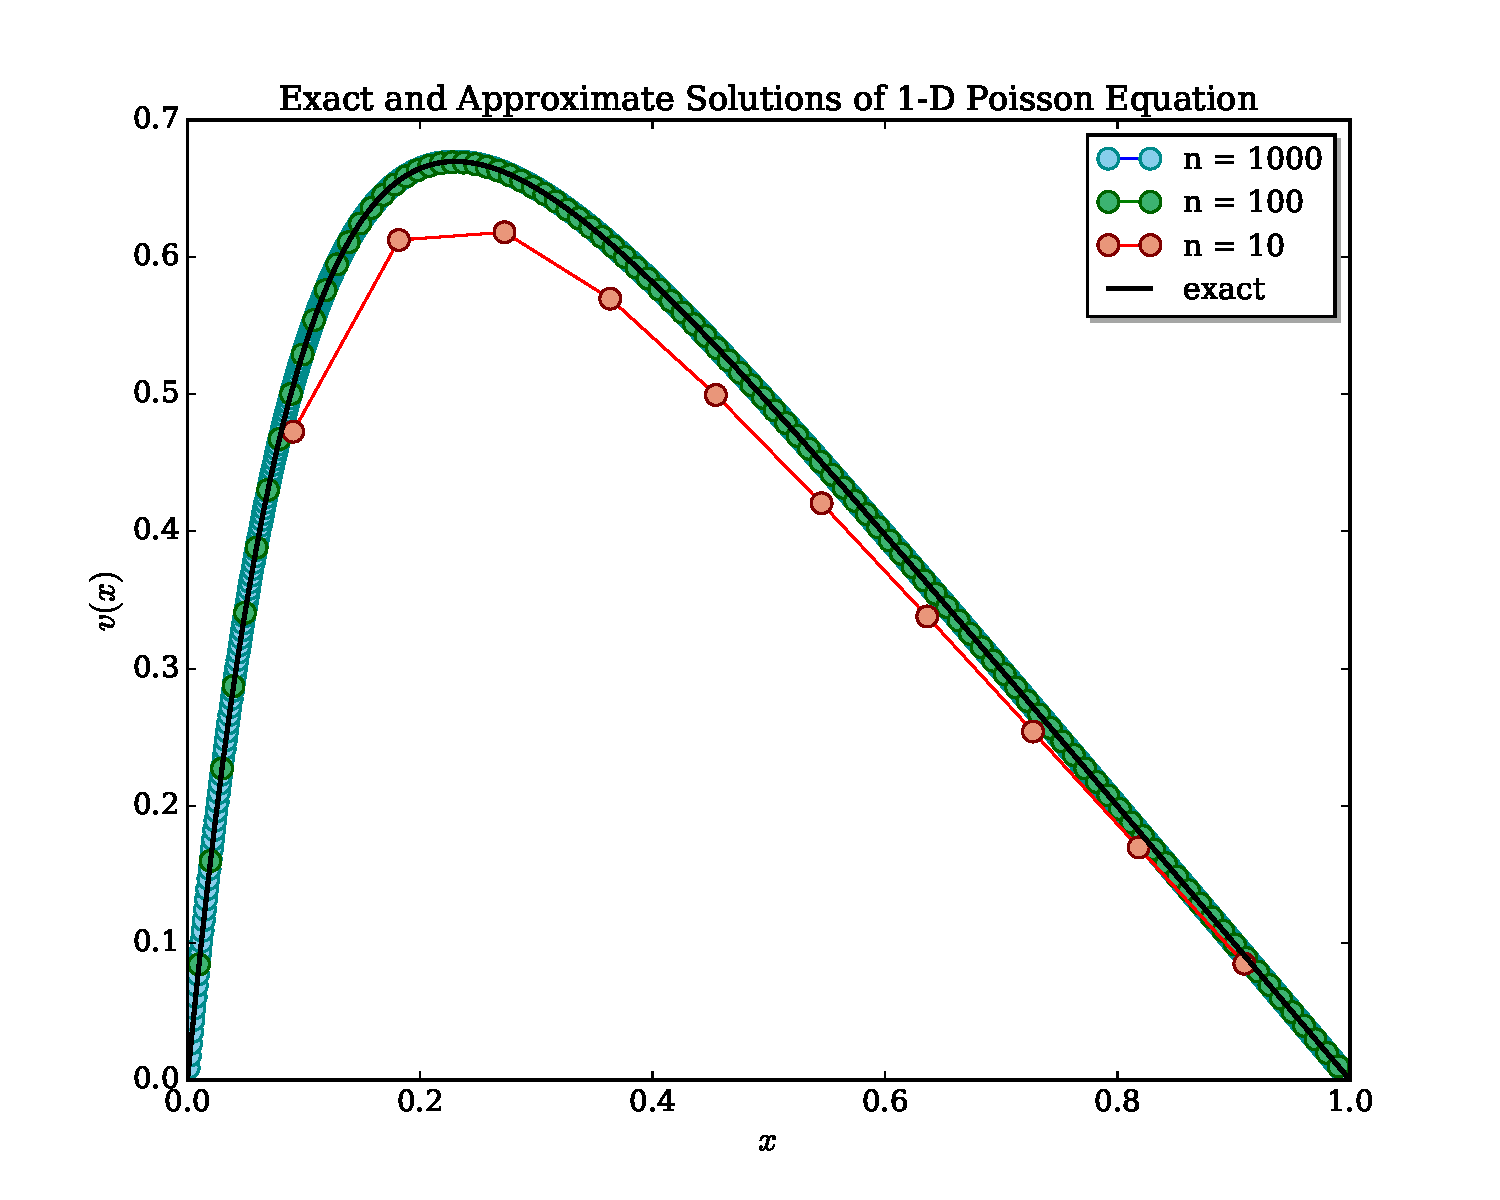
\includegraphics[scale=0.7]{compare_simple}
\end{figure*}
\textit{Figure 1.} The discretized solution $v_i$ for various $n$ are plotted alongside the closed-form solution $u(x)$. For $n>100$, the approximate and exact solutions are almost indistinguishable. 
\end{center}


discuss main finidings, link them up with existing literature, discuss eventual errors, effectiveness of your algorithm, stability of the calculations. 20 pts

The computation times for all four programs are shown in Table 1. 

\section{Conclusion}
summary of discussions and critical comments. 
what was learned about the methods i used? and results obtained? 
what about weird things when i was writing the code?
future improvements and possible directions?
comparison with iterative methods?
10pts\\

clarity of figures/overall presentation: 10 pts.
references: 5 pts

\newpage
blah biddy blah

\end{document}
